%@@@@@@@@@@@@@@@@@@@@@@@@@@@@@@@@@@@@@@@@@@@@@@@@@@
\chapter{Introduction}
\label{chap_Introduction}	
%@@@@@@@@@@@@@@@@@@@@@@@@@@@@@@@@@@@@@@@@@@@@@@@@@@

%#################################
\section{Problem overview}
%#################################
Images have fascinated humans for thousands of years.  The earliest cave paintings have been dated back to around 30,000 years \cite{2009_WEB_EarliestHumanPaintings_Gray}.  Currently, several fields deal with the creation and analysis of images.  Some example fields are art, photography, calligraphy and digital forensics.  In this work, we are primarily interested in the computational processing of images.  The three primary fields dealing with this aspect of images are Image Processing, Computer Vision and Computer Graphics.  The field of Image Processing deals with low level image analysis, Computer Vision deals with high level image analysis, and Computer Graphics primarily deals with image synthesis.  Within the field of Computer Vision, we are interested in tracking multiple objects in image sequences.

Object tracking, target tracking, or simply tracking, can be defined as estimating the trajectory of an object of interest over time.  In practical applications, tracking is normally preceded by a detection step and succeeded by a track analysis step \cite{2006_JNL_SURVEYtrk_Yilmaz}:

\begin{itemize}
\item \underline{Detection}.  In this step, objects of interest are identified and segmented.  A background model is commonly used as a pre-processing step.
\item  \underline{Tracking}.  The detected objects of interest are tracked from frame to frame.  
\item  \underline{Track analysis}.  In this step, track information is fused to infer higher semantic knowledge.
\end{itemize}

\begin{figure}[t]
	\center
	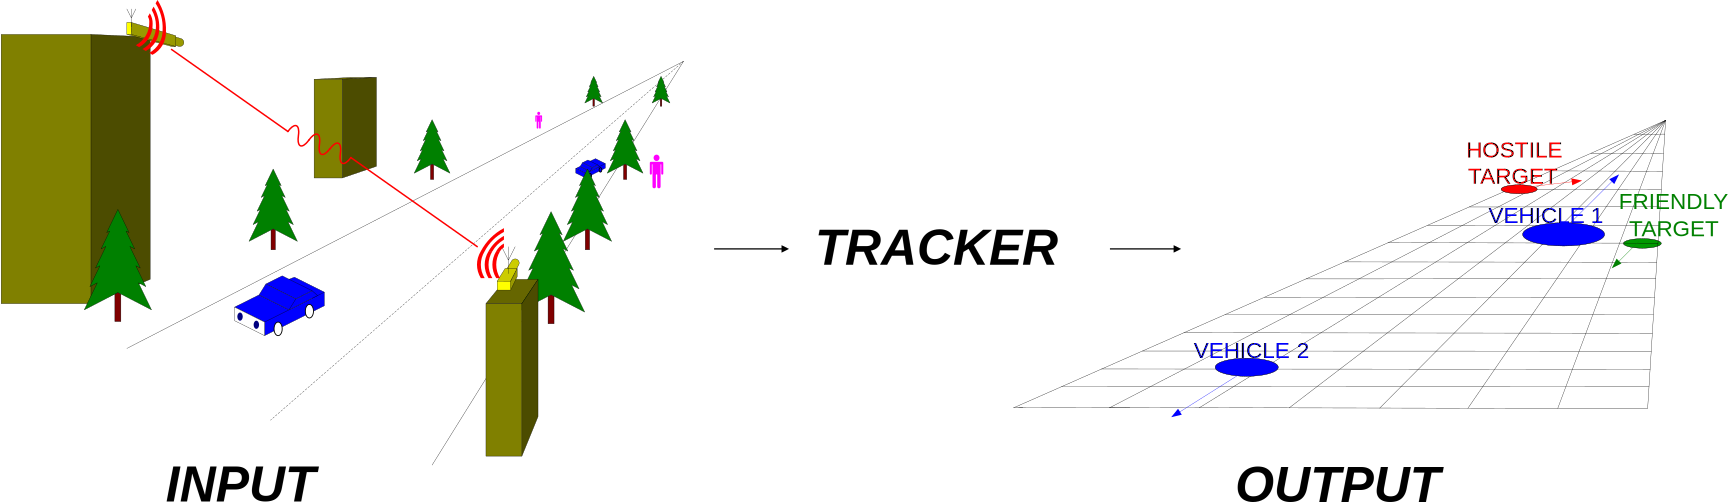
\includegraphics[width=1.1\textwidth]{thesis/TRK_overviewDiagram.pdf}
	\caption{Illustration of a visual tracking scenario.}
	\label{fig:TRK_illustration}
\end{figure}

Recently, there has been a surge in interest in tracking due to several reasons: (a) proliferation of powerful computers, (b) availability of high quality and inexpensive video cameras, and (c) an increasing need for automated video analysis.  However, in practice, many difficulties are encountered in visual tracking.  Some of these challenges include, 

\begin{itemize}
\item Loss of information caused by projecting 3D world objects onto 2D images
\item Sudden illumination changes
\item Appearance drifts
\item Complex target motion, including acceleration
\item Non-rigid or articulated nature of objects
\item Object-to-object merges/splits/occlusions
\item Object-to-scene occlusions
\item Camera motion
\item Noise
\item Real time processing requirements
\end{itemize} 

Clearly, visual tracking is a challenging problem.  Under general conditions, it remains an unsolved problem.  Several researchers have tried to approach this problem by specifying additional constraints on the targets being tracked.  Constraints have also been placed on the tracking environment.  For example, almost all tracking algorithms assume that the object motion is smooth without any abrupt changes \cite{2006_JNL_SURVEYtrk_Yilmaz}.  Furthermore, prior knowledge about the number, size, appearance and shape of the tracked objects has been used to simplify the problem.  

\begin{figure}[t]
	\center
	\includegraphics[width=1.0\textwidth]{thesis/2006_JNL_TRKsurvey_Shah_fig1.png}
	\caption{Target representations.  (a) Centroid, (b) multiple points,(c) rectangular bounding box, (d) elliptical bounding region, (e) articulated shape model, (f) skeleton, (g) contour control points, (h) contour, (i) silhouette \cite{2006_JNL_SURVEYtrk_Yilmaz}.}
	\label{fig:TRK_objectRepresentations}
\end{figure}

A graphical illustration of the tracking problem is shown in Figure~\ref{fig:TRK_illustration}.  In this figure, multiple cameras are employed for visual surveillance in an outdoor scenario.  The images captured by these cameras are fed to a tracker which returns metadata about the objects being tracked, such as target ID and target velocity.  Tracking is also commonly used in indoors applications, such as in tracking people in airports and malls.  Single camera tracking is also still widely used although multi-camera tracking is an active area of research.

%#################################
\section{Solutions}
%#################################
In the preceding section, we outlined the tracking scenario and some challenges faced therein.  We now turn to solutions.  

%===================
\subsection{Target representations}
%===================
Several algorithms have been employed for single and multiple target tracking.  The nature of the algorithm chosen is closely tied to the target representation.  Several target representations are shown in Figure~\ref{fig:TRK_objectRepresentations}.  

%===================
\subsection{Tracking algorithms}
%===================
The different target representations shown in Figure~\ref{fig:TRK_objectRepresentations} lend themselves to the following general categories of trackers:

\begin{itemize}
\item \underline{Point tracker}.  Targets represented using centroids or multiple points are commonly tracked using point trackers.  This form of tracking is closely tied to radar tracking.  As a matter of fact, the same techniques used in radar tracking are used.  Commonly used techniques include Kalman filtering, particle filtering~\cite{2002_JNL_PF_Arulampalam}, the \emph{probabilistic data association filter} (PDAF)~\cite{1975_JNL_PDAF_BarShalom}, the \emph{joint probabilistic data association filter} (JPDAF)~\cite{1983_JNL_JPDAF_Fortmann} and the \emph{multiple hypothesis tracker} (MHT)~\cite{1979_JNL_MTT_Reid}.
\item \underline{Region tracker}.  Targets represented using bounding boxes are commonly tracked using region tracking.  Widely used tracking methods in this category are template matching and mean shift tracking \cite{2002_JNL_MeanShift_Comaniciu}.
\item \underline{Contour tracker}.  Targets represented using shape information are commonly represented using splines and tracked using active contours \cite{2000_BOOK_ActiveVision_Blake} and level sets \cite{1995_JNL_LevelSets_Malladi}.
\end{itemize}

A closely associated problem is that of data association.  An overview of data association methods in target tracking is given in \cite{1993_JNL_SURVEYcorresp_Cox}.  More recently, particle filters have been shown to have an inherent capacity for data association \cite{1998_JNL_Condensation_IsardBlake}.   

%===================
\subsection{Preprocessing}
%===================
\begin{figure}[t]
	\center
	\fbox{
	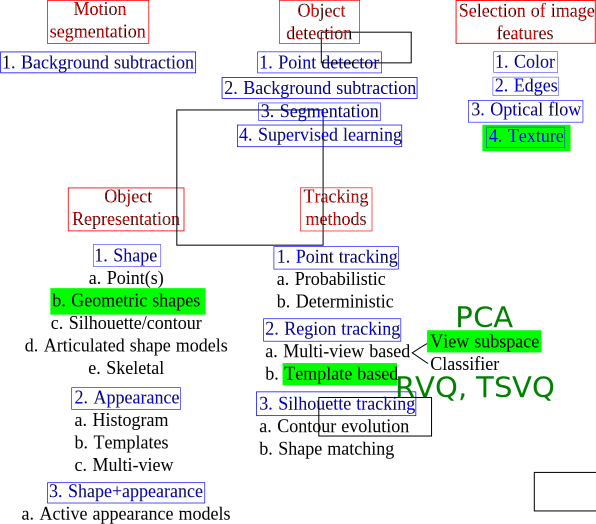
\includegraphics[width=1\textwidth]{thesis/TRK_overview.pdf}}
	\caption{Visual tracking, pre-processing steps, object representations and tracking methods~\cite{2006_JNL_SURVEYtrk_Yilmaz}.  In this work, we use the \emph{view subspace} method.}
	\label{TRK_overviewDiagram}
\end{figure}


It is common to apply pre-processing steps before tracking is initiated.  Some of these techniques include 

\begin{itemize}
\item \underline{Downsampling}.  This step is commonly carried out to reduce computational complexity.
\item \underline{Normalization}.  This step is commonly used to normalize brightness variation in temporal sequences.
\item \underline{Stabilization}.  Camera jitter is a common problem in tracking, especially in outdoor scenarios, or where cameras are hand-held.  Different camera stabilization algorithms have been proposed to reduce the effect of camera motion.  An overview can be found in \cite{2006_WHITE_stab_Sachs, 1999_JNL_stab_Engelsberg}.
\item \underline{Background modeling}.  Several methods have been suggested for background modeling.  A commonly used method is the multi-Gaussian algorithm \cite{1999_CNF_RealTimeTracking_Stauffer}.  An overview of background modeling methods can be found in \cite{1999_CNF_Wallflower_Toyama}.
\item \underline{Feature extraction}.  It is common to extract features from the target of interest and apply the algorithms mentioned above in the feature domain rather than in the raw spatial domain.  Commonly used features include color, edges, corners, motion, texture, depth and spatial intensity probability distribution.  For instance, corner detection \cite{1988_CNF_CombinedCornerEdgeDetector_Harris,2004_JNL_SIFT_Mikolajczyk} can be used to extract points of interest within the target which are then tracked using point trackers. 
\end{itemize}

An overview of these pre-processing steps, different object representations, and tracking methods is given in Figure~\ref{TRK_overviewDiagram}.

%#################################
\section{Current work}
%#################################
In this work, we use a technique called Residual Vector Quantization (RVQ) for tracking.  RVQ was first introduced in 1982 in the context of speech compression~\cite{1982_CNF_SpeechRVQ_JuangGray}.  The first application of RVQ for image analysis appeared in 2007 where this method was used to analyze damage caused by Hurricane Katrina in the United States~\cite{2007_JNL_Katrina_Barnes}.  Our work presents the first usage of RVQ for any form of video analysis. 

%#################################
\section{Outline}
%#################################
So far, we've briefly discussed three things in this introductory chapter: (a) the problem that we attempt to solve in this work, (b) the methods that have been employed in an attempt to solve this problem, and (c) the method that we intend to use in our own attempts.  The remaining portion of this document elaborates on these issues.  Here is an outline:

\begin{itemize}
\item \underline{Chapter 2.  Residual Vector Quantization}.  In this chapter, we discuss RVQ, give the mathematical notation involved, and discuss design, optimality and implementation issues.  A comparison with other vector quantization methods is also given.
\item \underline{Chapter 3.  Tracking methods}.  In this chapter, an overview of existing tracking methods is given.
\item \underline{Chapter 4.  RVQ tracking}.  In this chapter, visual tracking using RVQ is explained.  Comparison is also made with tracking using two well known methods, \emph{principal component analysis} (PCA) and \emph{tree-structured vector quantization} (TSVQ).  Six publicly available datasets are used that cover a variety of scenarios including indoors, outdoors, day-time, night-time, human, vehicle and object tracking, rigid and non-rigid object tracking, lighting change, structured noise, camera motion, target pose and expression changes, and temporary occlusions.  
\item \underline{Chapter 5.  Results}.  In this chapter, results of PCA, TSVQ and RVQ based tracking are presented and compared.
\item \underline{Chapter 6.  Conclusions}.  This chapter wraps up this thesis briefly restating objectives, summarizing results, presenting conclusions and laying out a ground map for future work.
\item \underline{Chapter 7.  Appendices}.  This chapter includes detailed plots for the interested reader.
\end{itemize}










